% Created 2018-04-16 Mon 16:01
% Intended LaTeX compiler: pdflatex
\documentclass[11pt]{article}
\usepackage[utf8]{inputenc}
\usepackage[T1]{fontenc}
\usepackage{graphicx}
\usepackage{grffile}
\usepackage{longtable}
\usepackage{wrapfig}
\usepackage{rotating}
\usepackage[normalem]{ulem}
\usepackage{amsmath}
\usepackage{textcomp}
\usepackage{amssymb}
\usepackage{capt-of}
\usepackage{hyperref}
\usepackage{listings}
\date{\today}
\title{Urschleim in Silicon: The Slideshow}
\hypersetup{
 pdfauthor={},
 pdftitle={Urschleim in Silicon: The Slideshow},
 pdfkeywords={},
 pdfsubject={},
 pdfcreator={Emacs 25.3.1 (Org mode 9.1.6)}, 
 pdflang={English}}
\begin{document}

\maketitle
\setcounter{tocdepth}{1}
\tableofcontents


\section*{Introductory Remarks}
\label{sec:org445b4ee}
\section*{The Concept of Return-Oriented Programming}
\label{sec:orgf0103e9}
\subsection*{The Fundamental Problem of Cybersecurity}
\label{sec:org11f693c}
At bottom, there is no essential distinction between data and code.

"Data" is just information your system trusts. 
\subsection*{Consider the Stack}
\label{sec:org0377207}
\begin{center}
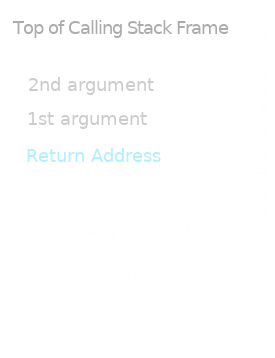
\includegraphics[width=.9\linewidth]{../images/stack_frame.png}
\end{center}
\begin{itemize}
\item the hacker feeds some input data to the process
\item which is written to a buffer in stack memory
\item but which overruns the buffer
\item corrupting the frame's return address
\end{itemize}

\subsection*{Consider the Stack, Smashed}
\label{sec:orgf6a182b}

\begin{center}
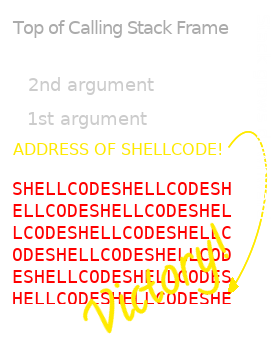
\includegraphics[width=.9\linewidth]{../images/stack_frame_attack.png}
\end{center}
\begin{itemize}
\item so that it points into the buffer
\item a buffer that turns out to contain machine code
\item to which the program counter "returns"
\item executing it just as it would its own instructions!
\end{itemize}

\subsection*{DEP / \(W \oplus X\)}
\label{sec:org2c772c5}
\begin{center}
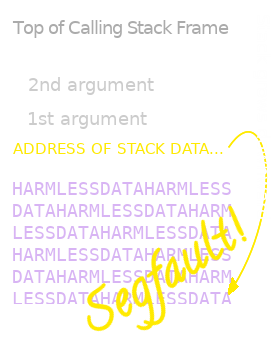
\includegraphics[width=.9\linewidth]{../images/stack_frame_attack_w^x.png}
\end{center}
\begin{itemize}
\item One way of mitigating this is to try to ensure that no page of memory is both writeable \textbf{and} executable.
\item The idea being that \emph{data} should be writeable, but never executable, while \emph{code} should be executed, but not written at runtime.
\end{itemize}



\subsection*{So, is code "wherever the program counter's pointing"?}
\label{sec:orga060a92}
\subsection*{No. It's far worse than that.}
\label{sec:orgc000ec0}
\subsection*{Subverting \(W\oplus X\)}
\label{sec:org4f4e5be}
\begin{itemize}
\item \(W\oplus X\) may prevent the \emph{execution} of input data, but it doesn't prevent attempts to \emph{return} to that data.
\item Why should the hacker need to supply their own machine code?
\item There's quite a bit just laying around, in executable memory.
\item Why not just build a payload with whatever's handy?
\end{itemize}
\subsection*{It's what MacGyver would do}
\label{sec:org8908343}
But how?
\subsection*{\(W\oplus X~~\) is a Leaky Abstraction}
\label{sec:org7769cc2}
\begin{itemize}
\item It rests on all-too-narrow concepts of "instruction" and "execution".
\item The payload's \emph{instructions} don't need to be bytes of machine code.
\item They just need to influence control flow, in a controllable way.
\end{itemize}
\subsection*{So is the \emph{Structured Programming Machine Model}}
\label{sec:org47e359b}
\begin{itemize}
\item The machine model structure programming is based already carves up an executable into chunks that \textbf{return} control after being dispatched.
\item To the programmer, these are "functions", but this is too granular a viewpoint.
\item \emph{Any} chunk of code ending with a \textbf{return} returns control to whomever controls the stack.
\item And our data controls the stack!
\end{itemize}

\subsection*{The ROVM supervenes on the SPMM}
\label{sec:org5ea4301}
\begin{itemize}
\item Chunks of code that allow the attacker to maintain control after dispatching are called "gadgets".
\item They can be seen as the instruction set for another virtual machine.
\item Call it a "Return-Oriented Virtual Machine".
\item It supervenes spontaneously on any process adhering to the SPMM.
\item It's a "weird machine"
\item and we can program it\ldots{}
\end{itemize}

\subsection*{\ldots{}and so can natural selection.}
\label{sec:org48ca03d}

\section*{Design and Implementation of ROPER}
\label{sec:org7ede115}

\section*{Experimental Studies}
\label{sec:org641a4b2}

\subsection*{The Environment}
\label{sec:orgcf5e03a}
\begin{center}
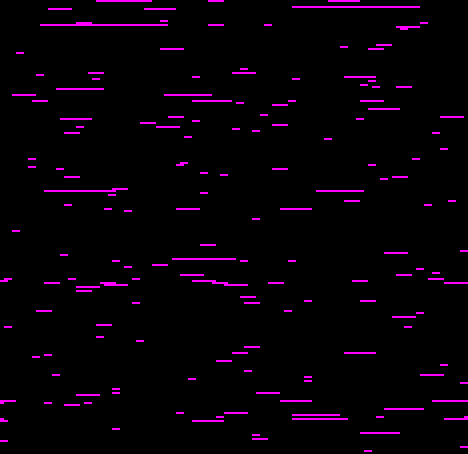
\includegraphics[width=.9\linewidth]{../../thesis/images/tomato-RT-N18U-httpd_heatmap.png}
\end{center}


\subsection*{Tasks and Fitness Functions}
\label{sec:orga3eacd6}
\begin{itemize}
\item An arbitrary and inscrutable fitness function
\item System call preparation
\item Classification tasks:
\begin{itemize}
\item An artificial, linearly-separable dataset
\item The Iris dataset
\end{itemize}
\item A Snake game
\end{itemize}



\subsubsection*{Kafka function with Crash Penalty}
\label{sec:org7d5beb1}

The address visitation heatmap shows no evident loss of diversity,
even after 212 seasons, suggesting a robustly ergodic system. 
\begin{center}
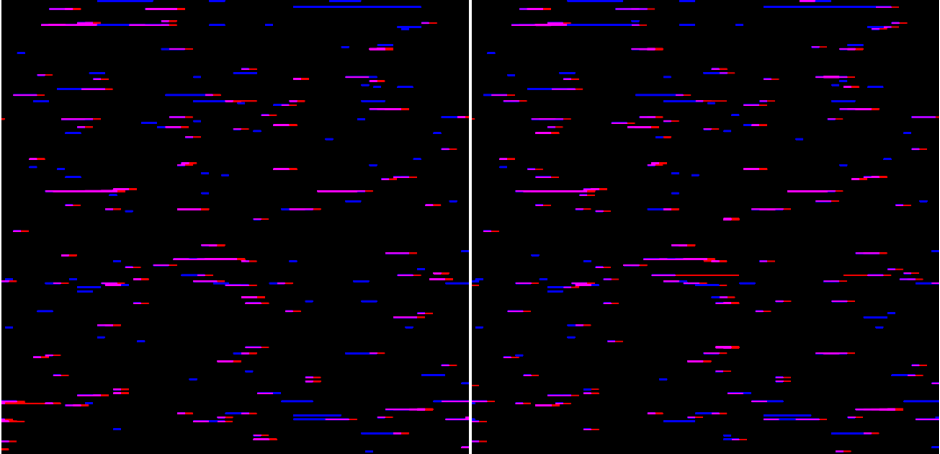
\includegraphics[width=.9\linewidth]{../../thesis/images/plots/xeqcyv_kafka_heatmap_beginning_end.png}
\end{center}


\subsubsection*{System Call Preparation}
\label{sec:org9f2d3e8}

Champion of the \emph{wiwzuh} population:
\lstset{language=asm,label= ,caption= ,captionpos=b,numbers=none}
\begin{lstlisting}
  0000b4ac        pop {r4, r5, r6, r7, r8, pc}

  0000d1a0        cmp r0, #0
  0000d1a4        popeq {r3, r4, r5, pc}

  00016654        cmp r0, #0
  00016658        ldr r3, [pc, #4]
  0001665c        moveq r0, r3
  00016660        pop {r3, pc}

  0001706c        ldm sp, {r0, r1}
  00017070        add sp, sp, #0x10
  00017074        pop {r4, r5, r6, pc}

;; R0:  0001f62f   R2:  00000000
;; R1: &0001f62f   R7:  0000000b

;; to call execv("/tmp/flashXXXXXX", ["/tmp/flashXXXXXX"], NULL) 
  00018fc4        svcvc #0xffffff
\end{lstlisting}


\subsubsection*{Fitness landscape traversed by the \emph{wiwzuh} population}
\label{sec:org872ceb9}
\begin{center}
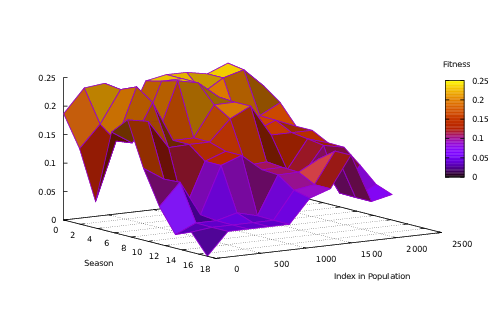
\includegraphics[width=.9\linewidth]{../../thesis/images/plots/wiwzuh_syscall_gaussian_3.png}
\end{center}



\subsubsection*{A simple classification task}
\label{sec:orga5db646}

\url{../images/plots/}

\subsubsection*{The Snake Game}
\label{sec:orgee24b79}

\url{../../videos/roper-snek-misjax-35000.mp4}

\section*{Recent and Future Work}
\label{sec:org8dc9a9a}

\subsection*{Recent}
\label{sec:orgd9a6995}

\subsubsection*{Bit-masks over Bid-bins}
\label{sec:org25a2554}

The uneven distribution of register usage puts a skew on any
classification task using the register bid-bin method. 
\begin{center}
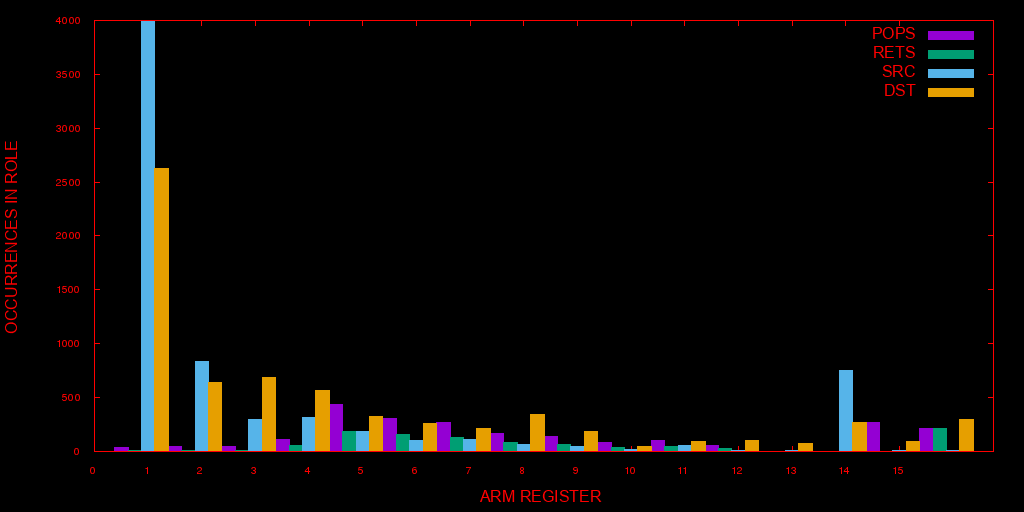
\includegraphics[width=.9\linewidth]{../images/tomato.png}
\end{center}

\subsubsection*{Bitmask technique for classification tasks}
\label{sec:org576f54e}



\subsubsection*{Specimens found when using the bitmask technique instead}
\label{sec:orgb6ed9b0}

\begin{verbatim}
IN:  a3 fffffd6f
0000b4b4       | pop {r4, r5, r6, r7, r8, pc}
0000d9a8       | cmp r0, #0
0000d9ac       | moveq r0, r3
0000d9b0       | pop {r3, pc}
0001010c       | rsb r5, r5, r0
00010110       | cmp r5, #0x40
00010114       | movgt r0, #0
00010118       | movle r0, #1
0001011c       | pop {r4, r5, r6, pc}
0000cdd0       | subs r4, r0, #0
0000cdd4       | popeq {r4, r5, r6, pc}
0000cdd8 stray | ldr r1, [pc, #0x1c]
0000cddc stray | mov r2, r4
0000cde0 stray | mov r0, #0
0000cde4 stray | bl #0x59e0
000127c4 stray | push {r1, r2, r3}
000127c8 stray | push {r0, r1, r2, r4, r5, r6, r7, r8, lr}
000127cc stray | mov r6, r0
000127d0 stray | mov r5, #0x400
000127d4 stray | add r7, sp, #0x28
000127d8 stray | ldr r8, [sp, #0x24]
000127dc stray | mov r0, r5
000127e0 stray | bl #4294933396
0000a374 stray | add ip, pc, #0
0000a378 stray | add ip, ip, #0x1e000
0000a37c stray | ldr pc, [ip, #0x5a8]!
0000a138 stray | str lr, [sp, #-4]!
0000a13c stray | ldr lr, [pc, #4]
0000a140 stray | add lr, pc, lr
0000a144 stray | ldr pc, [lr, #8]!
OUT: 400->0 1bc01->7365720a 1->7368732e 96106ace 1->7368732e 400->0 0->68732e00 
.... 2b02b->1 1bc01->7365720a 0->68732e00 0->68732e00 0->68732e00 28924->a138 2afff->127e4 28868->0 0->68732e00 
R0 (bin): 00000000000000000000010000000000
\end{verbatim}

\begin{verbatim}
IN:  ffffff98 d
0000b4b4       | pop {r4, r5, r6, r7, r8, pc}
0000d9a8       | cmp r0, #0
0000d9ac       | moveq r0, r3
0000d9b0       | pop {r3, pc}
0001010c       | rsb r5, r5, r0
00010110       | cmp r5, #0x40
00010114       | movgt r0, #0
00010118       | movle r0, #1
0001011c       | pop {r4, r5, r6, pc}
0000cdd0       | subs r4, r0, #0
0000cdd4       | popeq {r4, r5, r6, pc}
0000d9ac       | moveq r0, r3
0000d9b0       | pop {r3, pc}
00016168       | add r0, r4, r0
0001616c       | pop {r3, r4, r5, pc}
0000ad94       | mov r0, r3
0000ad98       | pop {r4, pc}
0001228c       | add sp, sp, #0x364
00012290       | add sp, sp, #0x400
00012294       | pop {r4, r5, r6, r7, r8, sb, sl, fp, pc}
OUT: ea->0 0->68732e00 ffffff98 ea->0 0->68732e00 0->68732e00 0->68732e00 
.... 0->68732e00 0->68732e00 0->68732e00 0->68732e00 0->68732e00 0->68732e00 2b7eb->0 0->68732e00 0->68732e00 
R0 (bin): 00000000000000000000000011101010
\end{verbatim}

\subsubsection*{TTL fields on Clumps}
\label{sec:orgc3144cb}

\subsubsection*{Quasi-Homologous Crossover}
\label{sec:org6510c59}

\subsection*{}
\label{sec:org701eb83}
\end{document}